% EBP course: session 5
% Thomas Klee
% 2019-02-20
% no changes from last year's lecture

% Preamble
\documentclass{beamer}
\usetheme{Singapore}
\usefonttheme[onlysmall]{structurebold}
\setbeamerfont{title}{shape=\itshape,family=\rmfamily}
\usepackage{graphicx}
\usepackage[english]{babel}
\usepackage[utf8x]{inputenc}
\usepackage{amsfonts, amsmath, amsthm, amssymb} % for math fonts, symbols and environments
\usepackage{xcolor}
\usepackage{booktabs}
\usepackage{ctable} % for command-driven tables
\usepackage{wasysym}
\usepackage[natbibapa]{apacite}
\beamertemplatenavigationsymbolsempty % uncomment to add slide navigation symbols to each slide
\setbeamertemplate{footline}[frame number]
\usepackage{appendixnumberbeamer}  % to suppress page numbers on extra slides

% activate following line for custom appearance
% \usepackage{beamerthemesplit} 

\mode<presentation>

% information for title slide
\title{Cohort and Case-Control Studies}
\subtitle{}
\author{Evidence-Based Practice in Speech-Language Therapy \\ (SHSC 2033)}
\institute{Session 5}
\date{Thomas Klee \& Elizabeth Barrett}
\titlegraphic{
\includegraphics[width=6cm]{images/logo_CE_C.jpg}} % HKU logo

\begin{document}

% create title slide with information above
\begin{frame}
	\titlepage
\end{frame}

% 1
\begin{frame}{Outline}
	\begin{enumerate}
	\item Cohort studies
	\item Case-control studies
	\item Useful tools
	\item Group discussion
	\end {enumerate}
\end{frame}

% 2
\begin{frame}{Introduction}
	\begin{itemize}
	\item RCTs are \textbf{experimental studies}. They're designed with a high degree of experimental control built in. 
	\item Other kinds of evidence comes from \textbf{non-experimental studies}, where there's been no experimental manipulation of participants---and more possibilities for bias and confounds. These are a kind of \textbf{observational study}.
	\item Cohort studies and case-control studies are two kinds of observational studies where naturally occurring events (hypothesized risks, exposures) are observed.
	\item These are employed in studies of \textbf{epidemiology} and sometimes in intervention.
	\end {itemize}
\end{frame}

\section{Cohort Studies}

\begin{frame}
\begin{center}
\Huge{Cohort Studies}
\end{center}
\end{frame}

% 3
\begin{frame}{What is a cohort study?}
	\begin{itemize}
	\item ``\dots the investigator identifies exposed and nonexposed groups of patients, each in a cohort, and then traces their outcome forward in time."\footnote{\tiny{\citet[p. 147]{Guyatt2008d}}}
	\item Usually prospective but can be retrospective
	\item Observational rather than experimental
	\item Longitudinal rather than cross-sectional
	\item (Relative) risk ratios calculated to estimate risk of the exposure
	\end{itemize}
\end{frame}

% US NLM definition
%\begin{frame}{What is a cohort study?}
%	\begin{itemize}
%	\item An observational study in which outcomes in a group of patients that received an intervention are compared with outcomes in a similar group (i.e., the cohort, either contemporary or historical) of patients that did not receive the intervention\footnote{\tiny{\url{https://www.nlm.nih.gov/nichsr/hta101/ta101014.html}}}
%	\end{itemize}
%\end{frame}

% CEBM definition
%\begin{frame}{What is a cohort study?}
%	\begin{itemize}
%	\item The analytic method of epidemiologic study in which subsets of a defined population can be identified who are, have been, or in the future may be exposed or not exposed, or exposed in different degrees, to a factor or factors hypothesized to influence the probability of occurrence of a given disease or other outcome. The main feature of cohort study is observation of large numbers over a long period (commonly years) with comparison of incidence rates in groups that differ in exposure levels.\footnote{\tiny{\url{http://www.cebm.net/glossary/}}}
%	\end{itemize}
%\end{frame}

% 4
\begin{frame}{Cohort studies}
	\begin{itemize}
	\item Most are \textbf{prospective}: the study begins and individuals are followed until the outcomes (events of interest) occur. 
	\item Some are \textbf{retrospective}: ``the outcomes (events of interest) have already happened at some point in the past; the investigator simply goes back even farther in the past and selects exposed and unexposed people; then the question is whether these differ in the development of the outcomes of interest."
	\footnote{\tiny{\citet[p. 147]{Guyatt2008d}}}
	\end{itemize}
\end{frame}

% 5
\begin{frame}{Cohort study}
\begin{center}
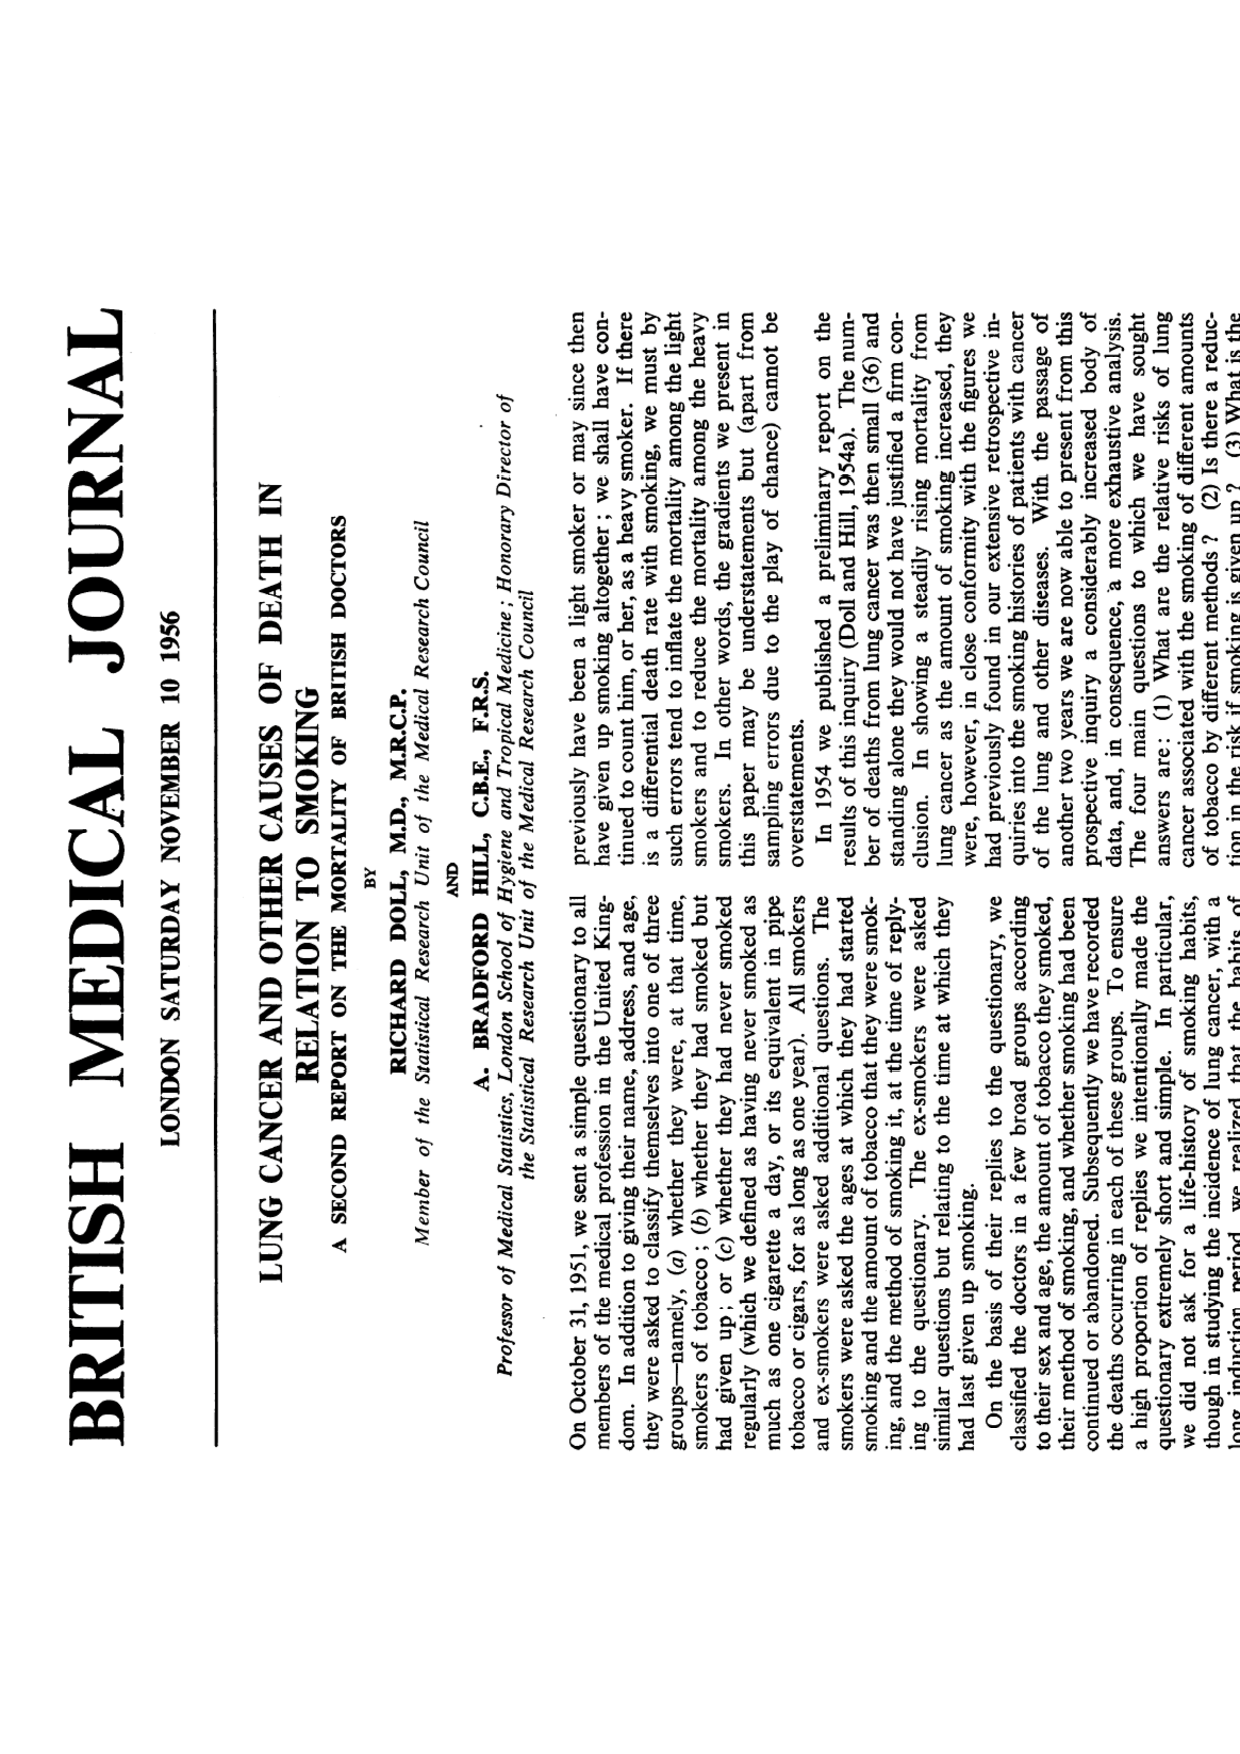
\includegraphics[angle=270, origin=c, width=10cm]{images/dollHill1956.pdf}
\end{center}
\end{frame}

% 6
\begin{frame}{Cohort study \citep{Doll1956}}
	\begin{itemize}
	\item Research question: What are the relative risks of lung cancer associated with smoking?
	\item Questionnaires were sent to all doctors in the UK in October 1951 (so the \textbf{cohort} was doctors).
	\item Doctors were asked whether they smoked and were classified into non-smokers, present smokers, and ex-smokers.
	\item Subsequent deaths were recorded in each group for the next 4 years, 5 months.
	\item Prospective, longitudinal study
	\end{itemize}
\end{frame}

% 7
\begin{frame}{Cohort study methods \citep{Doll1956}}
	\begin{itemize}
	\item Questionnaires were sent to 59,600 doctors; 41,024 were completed.
	\item 40,701 were sufficiently complete to be used.
	\item 1,854 subsequent deaths were recorded during the period (1,714 over age 35) and the cause of death was noted.
	\end{itemize}
\end{frame}

% 8
\begin{frame}{Cohort study results\footnote{\tiny{Adapted from \citet[Table V, p. 1073]{Doll1956}.}}}
	\begin{table} % all the tables are formatted for use with the booktabs package
	\centering
	\begin{tabular}{ l c c c }
	\toprule
	Cause of death & No. deaths & Non-smokers$^3$ & All smokers\footnote{\tiny{Standardized death rates per year per 1,000 men aged 35 or more.}} \\
	\midrule
	Lung cancer & 84 & \alert{0.07} & \alert{0.90} \\
	Other cancer & 220 & 2.04 & 2.02 \\
	Other respiratory & 126 & 0.81 & 1.13 \\
	Coronary thrombosis & 508 & 4.22 & 4.87 \\
	Other causes & 779 & 6.11 & 6.89 \\
	\midrule
	All causes & 1,714 & 13.25 & 15.78 \\
	\bottomrule
	\end{tabular} 
%	\caption{$^*$Standardized death rates per year per 1,000 men aged 35 or more.} 
	\end{table}
\end{frame}

% 9
\begin{frame}{Cohort study results \citep{Doll1956}}
	\begin{itemize}
	\item The risk of lung cancer in smokers was found to be about \alert{13 times} that of non-smokers. (Risk ratio\footnote{\tiny{Also known as \textbf{relative risk}.}} = $0.90 / 0.07= 12.9$) 
	\item Threats to \textbf{external validity}:
		\begin{itemize}
		\item[-] Be careful not to over-generalize these results. 
		\item[-] They're based on male doctors (not the general population) and only those who responded to the questionnaire.
		\item[-] Participants weren't randomized to smoking and non-smoking groups, so confounds may have been present.
		\item[-] They're based on a previous generation of people. (Think of advances in health care, etc.) 
		\end{itemize}
	\end{itemize}
\end{frame}

% 10
\begin{frame}{Levels of evidence for intervention studies\footnote{\tiny{\url{http://www.cebm.net/index.aspx?o=1025}}}}
	\begin{itemize}
	\item[1a] Systematic reviews (SR) \& meta-analyses (with homogeneity) of RCTs
	\item[1b] Individual RCT (with narrow confidence interval)  
	\item[2a] \alert{SR (with homogeneity) of cohort studies}
	\item[2b] \alert{Individual cohort study (including low quality RCT)}
	\item[3a] SR (with homogeneity) of case-control studies
	\item[3b] Individual case-control studies
	\item[4] Case-series (and poor quality cohort and case-control studies)
	\item[5] Expert opinion without explicit critical appraisal; bench research
	\end{itemize}
\end{frame}

% 11
\begin{frame}{Another example}
	\begin{itemize}
	\item The ``Growing up in New Zealand" study\footnote{\tiny{\url{http://www.growingup.co.nz/en/about-the-study.html}}}
	\item Designed to ``to improve the lives of their generation and answer the fundamental question: What makes us who we are?"
	\item A pre-birth cohort study
	\item 7,000 children being followed from before birth to early adulthood (21 years planned)
	\end{itemize}
\end{frame}

\section{Case-Control Studies}

\begin{frame}
\begin{center}
\Huge{Case-Control Studies}
\end{center}
\end{frame}

% 12
\begin{frame}{What is a case-control study?}
``Case-control studies also assess associations between exposures and outcomes. \dots [they provide] an alternative design that relies on the initial identification of \alert{cases}---that is, patients who have already developed the target outcome---and the selection of \alert{controls}---persons who do not have the outcome of interest."
\footnote{\tiny{\citet[p. 146]{Guyatt2008d}}}

\end{frame}

% 13
\begin{frame}{Case-control studies}
	\begin{itemize}
	\item People with a condition (cases) are compared to those without the condition (controls) with regard to putative risk factors or exposures.
	\item Usually retrospective; observational
	\item Usually less expensive and quicker to do than a cohort study
	\item Odds ratios (ORs) are calculated to estimate risk (see handout on Moodle).
	\end{itemize}
\end{frame}

% 14
\begin{frame}{Case-control study}
\begin{center}
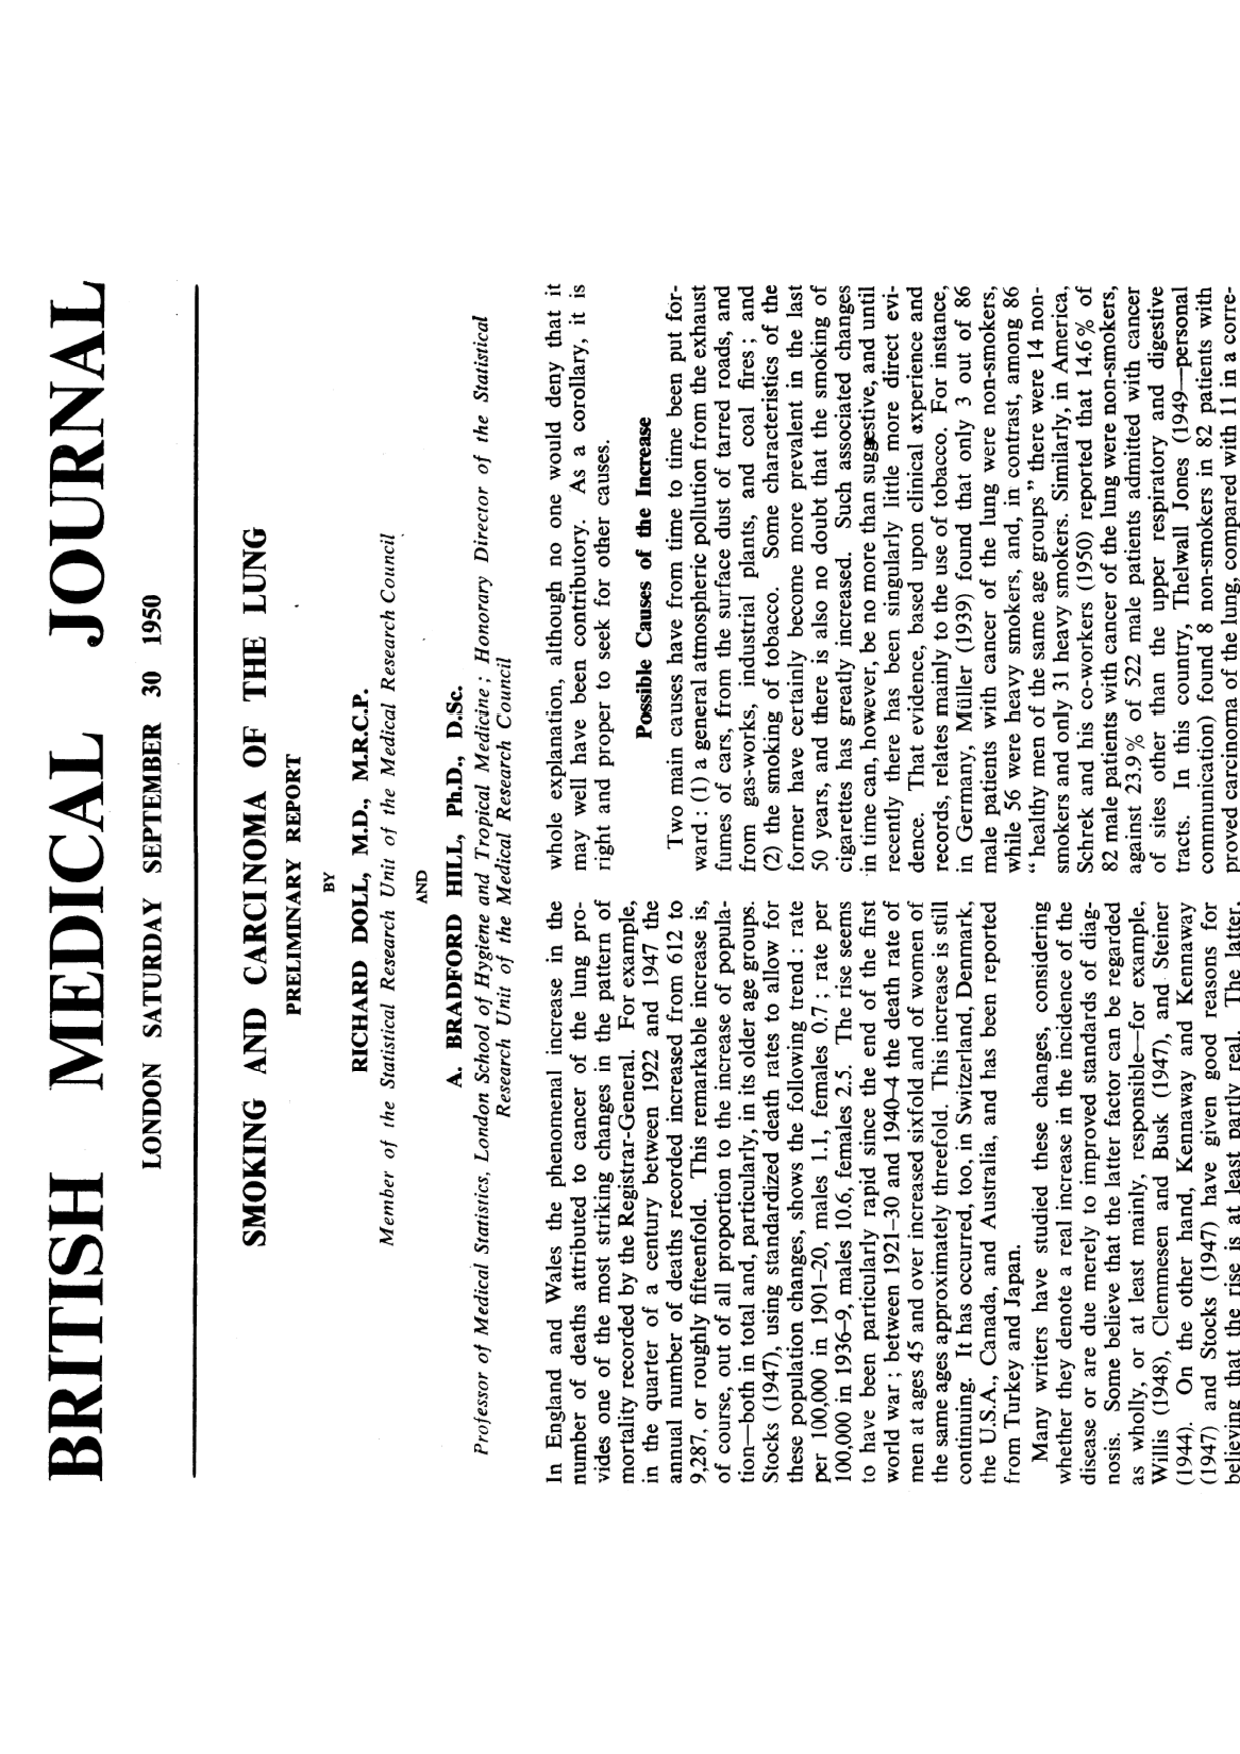
\includegraphics[angle=270, origin=c, width=10cm]{images/dollHill1950.pdf}
\end{center}
\end{frame}

% 15
\begin{frame}{Case-control study \citep{Doll1950}}
	\begin{itemize}
	\item ``\dots to determine whether patients with carcinoma of the lung differed materially from other persons in respect of their smoking habits or in some way which might be related to the atmospheric pollution theory." (p. 740)
	\item 20 London hospitals were asked to notify all patients admitted with carcinoma of the lung \alert{(cases)}.
	\item For each case, researchers also interviewed a \alert{control} patient from a group of non-cancer patients of the same sex, within the same age group, and in the same hospital at about the same time. 
	\item Case and control patients were interviewed using a questionnaire and asked about their smoking history.\footnote{\tiny{A smoker was defined ``as a person who had smoked as much as one cigarette a day for as long as one year."}}
	\item Retrospective study
	\end{itemize}
\end{frame}

% 16
\begin{frame}{Case-control study results \citep{Doll1950}\footnote{\tiny{Results for male patients. Adapted from Table IV of study and from \citet[p. 242]{Bland2000}.}}}
	\begin{table}
	\centering
	\begin{tabular}{ l c c c }
	\toprule
	& Smokers & Non-smokers & Total\\
	\midrule
	Lung cancer & 647 & 2 & 649 \\
	Controls & 622 & 27 & 649 \\
	\bottomrule
	\end{tabular} 
	\end{table}
\end{frame}

% 17
\begin{frame}{Case-control study results \citep{Doll1950}}
	\begin{itemize}
	\item In case-control studies, relative risk is approximated by the \textbf{odds ratio}: $(647 / 2) / (622 / 27)= 14.04$ \footnote{\tiny{\citet[p. 242]{Bland2000}}} 
	\item The risk of lung cancer in smokers is about \alert{14 times} that of non-smokers.  
	\item The 95\% CI is wide \alert{[3.3, 59.3]} due to the small number of non-smokers, particularly for lung cancer cases.\footnote{\tiny{\citet[p. 243]{Bland2000}}}
	\item Consider threats to external validity
	\end{itemize}
\end{frame}


% 18
\begin{frame}{Smoking and lung cancer}
	\begin{block}{Initial study}
Doll and Hill's \alert{case-control study} of 1950 concluded that the risk of lung cancer in male smokers is about 14 times that of non-smokers.\footnote{\tiny{\citet[pp. 241--242]{Bland2000}}}
	\end{block}
	\begin{block}{Subsequent study}
In their \alert{cohort study} of 1956, they reported a similar finding (risk about 13x higher in smokers).\footnote{\tiny{Bland uses the term \emph{risk} in summarising the findings, although the number was an OR.}}
	\end{block}
\end{frame}

% 19
\begin{frame}{Levels of evidence for intervention studies\footnote{\tiny{\url{http://www.cebm.net/index.aspx?o=1025}}}}
	\begin{itemize}
	\item[1a] Systematic reviews (SR) \& meta-analyses (with homogeneity) of RCTs
	\item[1b] Individual RCT (with narrow confidence interval)  
	\item[2a] SR (with homogeneity) of cohort studies
	\item[2b] Individual cohort study (including low quality RCT)
	\item[3a] \alert{SR (with homogeneity) of case-control studies}
	\item[3b] \alert{Individual case-control studies}
	\item[4] Case-series (and poor quality cohort and case-control studies)
	\item[5] Expert opinion without explicit critical appraisal; bench research
	\end{itemize}
\end{frame}

% 20
\begin{frame}{Risk factors for late talking\footnote{\tiny{$N = 1766$, of which 238 were LTs, defined using Communication scale of the Ages and Stages Questionnaire at 2.1 years of age \citep[Table 3]{Zubrick2007}; adjusted ORs reported.}}}
	\begin{table}
	\centering
	\begin{tabular}{ l c c }
	\toprule
	Risk factor & Odds ratio & 95\% CI \\
	\midrule
	Male sex & 2.74 & [1.96, 3.84] \\
	Family history of late talking & 2.11 & [1.40, 3.19] \\
	Two or more children in family & 2.08 & [1.39, 3.10] \\
	Early neurobiological growth & & \\
	- Percent optimal birth weight $<85\%$ & 1.89 & [1.18, 3.02] \\
	- Prematurity $\leq 36$ weeks & 1.84 & [1.04, 3.25] \\
	- Gross motor skills (ASQ) & 3.12 & [1.30, 7.52] \\
	- Fine motor skills (ASQ) & 2.39 & [1.20, 4.78] \\
	- Adaptive skills (ASQ) & 2.65 & [1.66, 4.22] \\
	- Personal-social skills (ASQ) & 5.53 & [2.06, 14.87] \\
	\bottomrule
	\end{tabular} 
	\end{table}
\end{frame}

% 21
\section{Useful Tools}

\begin{frame}{Useful tools for cohort and case-control studies}
	\alert{Reporting standards for authors (STROBE)} \url{http://www.equator-network.org}
	
\vspace{3mm}
	\alert{Critical appraisal checklists for readers (SIGN)} \url{http://www.sign.ac.uk/checklists-and-notes.html}
	
\vspace{3mm}
	\alert{Relative risk calculator} \url{https://www.medcalc.org/calc/relative_risk.php}

\vspace{3mm}
	\alert{Odds ratio calculator} \url{https://www.medcalc.org/calc/odds_ratio.php}
\end{frame}

\section{Group Discussion}

%22
\begin{frame}{Press Release\footnote{\tiny{HKU Daily Media Highlights, 2018-02-11}}}
\textbf{Medical experts refute singers' claims of flu vaccine risks}
\\
\vspace{3mm}
\footnotesize{``Cantopop singers have recently made warnings against flu vaccines. In a leaked WhatsApp audio recording, Ms Kay Tse On-kei said flu vaccines contained mutated bacteria and mercury. [Her] claims were rejected by HKU microbiologist Professor Yuen Kwok-Yung. Dr Ho Pak Leung, Director of the HKU Centre for Infection, \dots emphasized that medical issues should be separated from entertainment. HKU Dean of Medicine Professor Gabriel Leung said these comments made by well-known figures had no support from the scientific and medical fields. \\
\vspace{3mm}
HKU released findings of a study on the effectiveness of the vaccine type for the current flu season. It found that the flu jabs were 66\% effective. The study looked into the data of 1,078 children who were admitted to hospitals between December 4 last year and January 31 this year. All the children suffered from fever and acute respiratory illness. Among the 339 confirmed with flu, only 22 had been vaccinated. Of the remaining 739 children who were unaffected by the virus, 103 had received seasonal flu vaccinations. (Major local papers)"}
\end{frame}

% 23
\begin{frame}{Group discussion}
	\begin{itemize}
	\item Break up into your assigned groups.
	\item Decide whether the flu vaccine has been effective in Hong Kong based on the data in the press release.  
	\item Use SIGN checklist 4 for case-control studies to critically appraise the research article.
	\item Document \alert{where} you found information addressing each point.
	\item Upload checklist for your group by 11.45am.
	\end{itemize}
\end{frame}

\begin{frame} [shrink=15] % to reduce font size of references; *comment out this part first time this is run* 
	\frametitle{References}
	\bibliographystyle{apacite}
	\small\bibliography{/Users/thomasklee/Documents/Bibtex/library}
\end{frame}

\end{document}